\chapter{Documentos de Viaje}\label{apendix:DocDeViaje}

%%%%%%%% TIPOS DE DOCUMENTOS 
\section{Tipos de documentos de viaje}\label{subsec:TiposDocumentosDeViaje}

Existe distintos documentos que permiten el cruce de fronteras, pero no todos pueden procesarse de manera automática, para ello deben cumplir la normativa fijada para los \textbf{\gls{eMRTD}} en \textbf{\GLS{ICAO}-Doc $9303$} \cite{doc20069303}. Esta normativa ofrece estándares para distintos documentos de identificación personal: \textit{Electronic Driver's License} (\textbf{\gls{eDL}}), \textit{Electronic Passport} (\textbf{\gls{e-passport}}), \textit{Electronic Vehicle Registration Card} (\textbf{\gls{eVRC}}), \textit{Electronic Visa} (\textbf{\gls{eVISA}}), \textit{Electronic Identity} (\textbf{\gls{eID}}), \textit{Electronic Residence Permit} (\textbf{\gls{eRP}}). Pero los documentos que comúnmente procesan los sistemas \GLS{ABC} son: \textbf{\gls{e-passport}}, \textbf{\gls{eVISA}} y en algunos países el \textbf{\gls{eID}}.

\medskip
\textbf{\gls{e-passport}}

Es el documento más habitual para la identificación en los cruces de frontera.

La \textbf{información de la identidad} se encuentra en la hoja de datos en la \textit{Visual Inspection Zone} (\textbf{\GLS{VIZ}} Figura \ref{fig:HojaDatos_MRZ} (a)) y en la \textit{Machine Readable Zone} (\textbf{\GLS{MRZ}} Figura \ref{fig:HojaDatos_MRZ} (b)).

Paralelamente, toda la información también se alanaceba en un chip, un circuito integrado leíble por radio frecuencia, \textit{Radio Frequency Identification} \textbf{\GLS{RFID}} en el que también se almacenan uno o varios rasgos biométricos encriptados con \textit{Public Key Infraestructure} (\textbf{\GLS{PKI}}), cuya clave de encriptación es gestionada por el país emisor.

Los rasgos biométricos recomendado por \GLS{ICAO} son la \textbf{cara}, las \textbf{huellas dactilares} y el \textbf{\gls{iris}}. Pero, aunque todos los países almacenan una imagen de la cara, sólo algunos almacenan dos imágenes con la huellas dactilares y muy pocos, imágenes con el \gls{iris} de ambos ojos \footnote{En el caso de España si se trata de un \gls{e-passport} de primera generación sólo una imagen de la cara, si es de segunda generación además de la cara, una imagen de las huellas dactilares.}. 

\medskip
\textbf{\gls{eVISA}}

Es un tipo de documentación requerido para la entrada en ciertos países y algunos sistemas \GLS{ABC} ya están preparados para leerlos. 

Como el \gls{e-passport}, tiene una zona de inspección visual \textbf{\GLS{VIZ}} y otra de lectura automática \textbf{\GLS{MRZ}} con los datos de la identidad del viajero y también puede contener datos biométricos como las huellas dactilares. 

La información de estos documentos debe ser verificada contra una base de datos \textit{Visa Information System} (\textbf{\GLS{VIS}}). 

\begin{figure}[ht]
    \centering
    \includegraphics[width=1.\textwidth]{ch-sistemasABC/images/ch-SistemasABC/CARNET_IDENTIDAD_ESPAÑOL_ALEMAN.png}
    \caption{Documentos de identificación nacional a) Español (\gls{DNI-e}) b) Alemán (\textit{\gls{Personalausweis}}).}
    \label{fig:DocIdentidadNacional}
\end{figure}

\medskip
\textbf{\Gls{nacional-ID}}

Actualmente muy pocos sistemas \GLS{ABC} son capaces de procesar este tipo de documentos, ya que su formato viene fijado por las reglas de cada país y sólo algunos países se ajustan al estándar \textbf{\gls{eID}} de \GLS{ICAO} \cite{doc20069303}, como España (Figura \ref{fig:DocIdentidadNacional} (a)) o Alemania (Figura \ref{fig:DocIdentidadNacional} (b)) que almacenan rasgos biométricos en este tipo de documentos. 

\begin{landscape}
 \begin{figure}
  \centering
  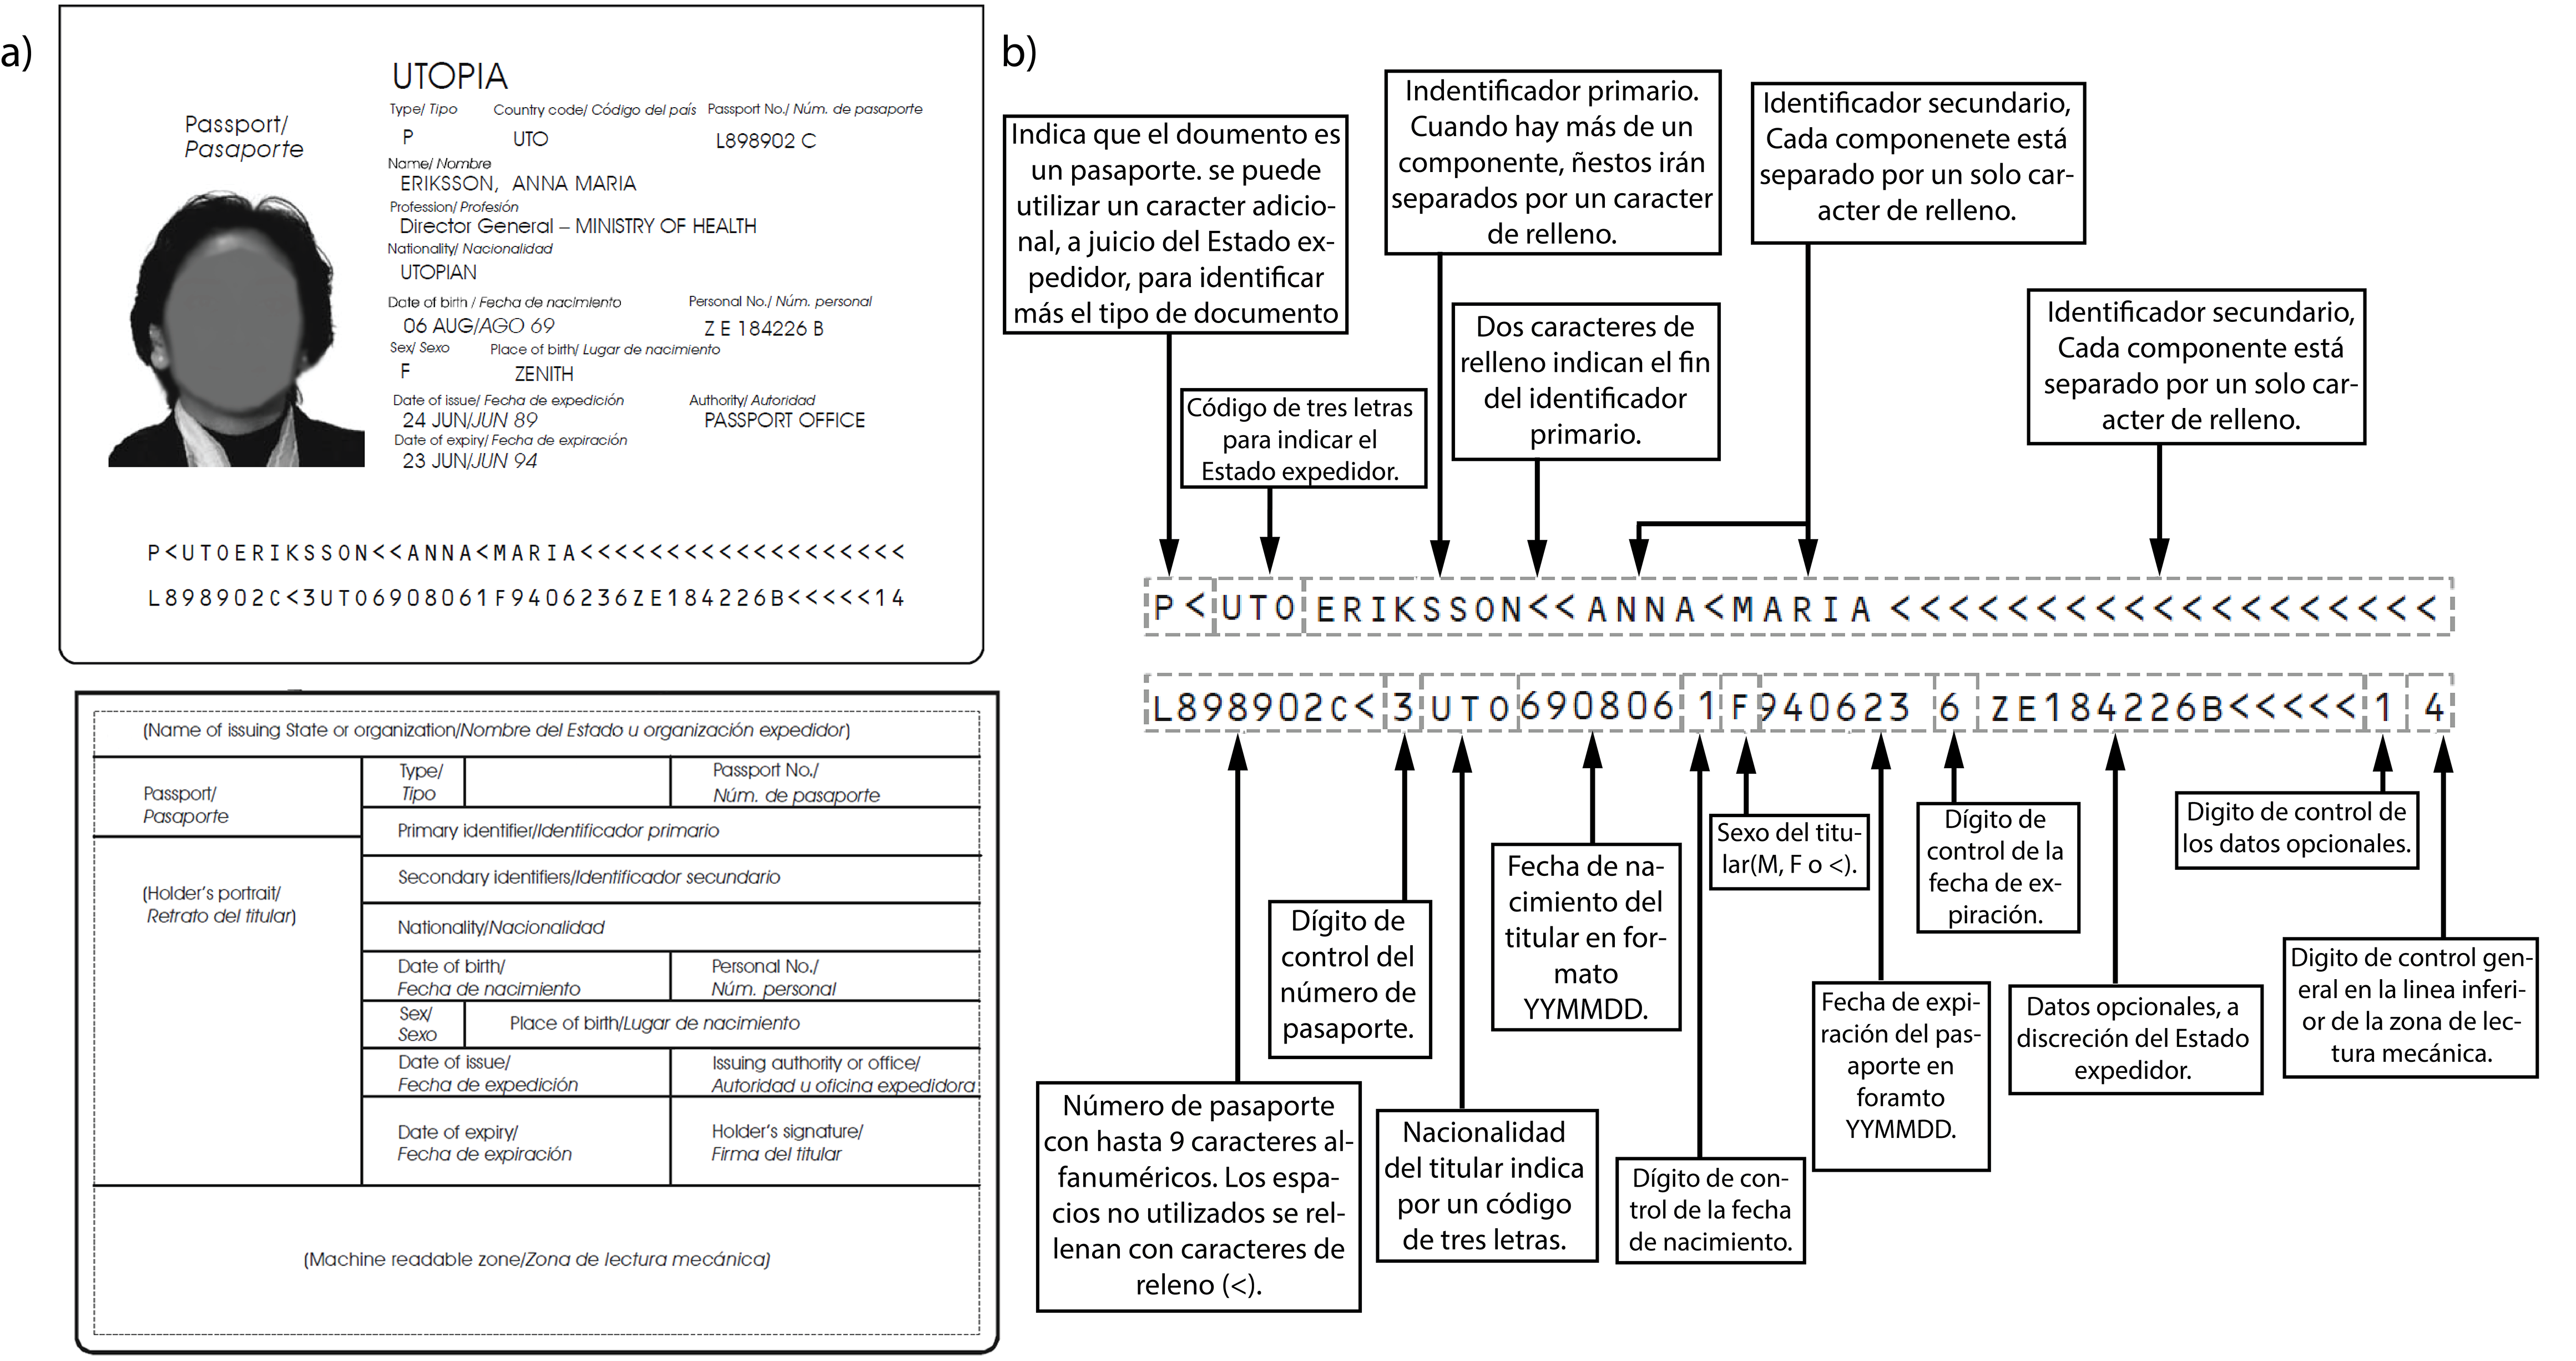
\includegraphics[scale=0.6]{ch-sistemasABC/images/ch-SistemasABC/HOJA_DE_DATOS_Y_MRZ_DEL_PASAPORTE.png}
  \caption{a) Hoja de la datos y b) \textit{Machine-Readable Zone} (\GLS{MRZ}) de los \textit{\gls{e-passport}}, definida en el informe \GLS{ICAO} Doc $9303$ \cite{doc20069303}.}
  \label{fig:HojaDatos_MRZ}
\end{figure}
\end{landscape}


%%%%%%%% SEGURIDAD DE DOCUMENTOS 
\begin{figure}
  \centering
  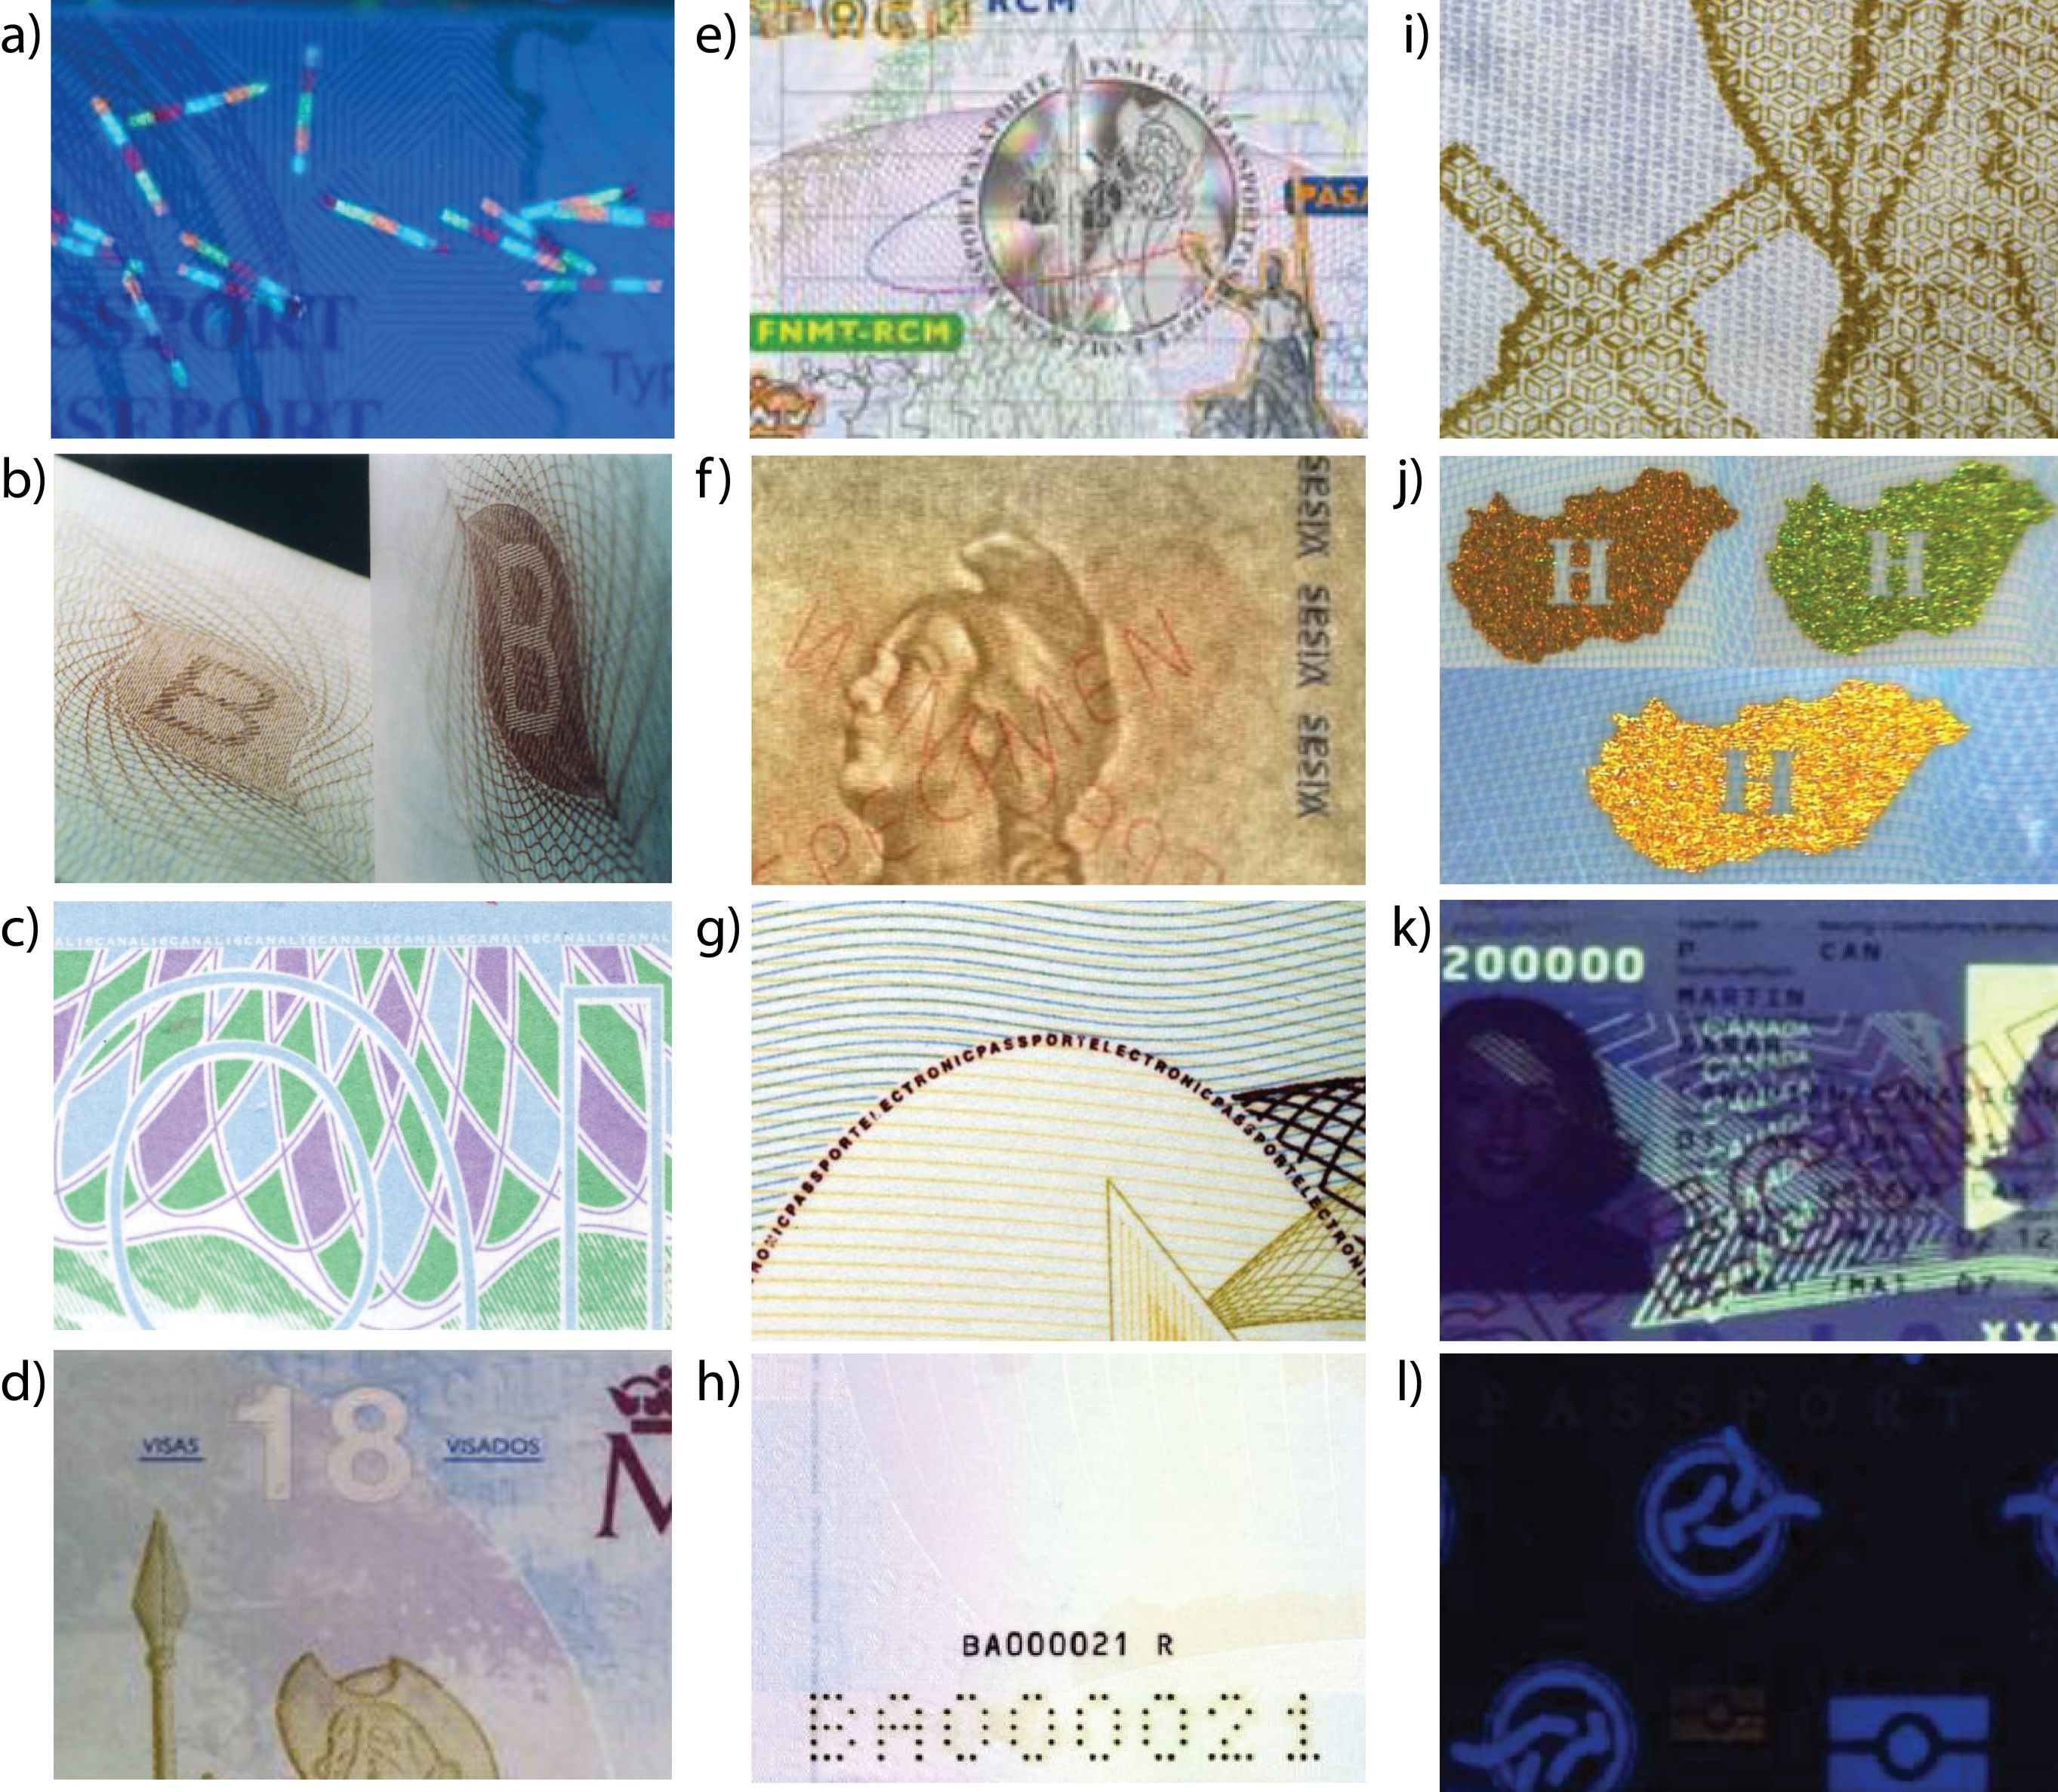
\includegraphics[width=1\textwidth]{ch-sistemasABC/images/ch-SistemasABC/MEDIDAS_SEGURIDAD_EN_PASAPORTES.png}
  \caption{Marcas de seguridad habituales en los documentos de viaje: a)Papel con fibras invisibles. b)Imágenes latentes. c)Guillones de distintos colores. d)Impresión offset de seguridad. e)Láminas holográficas. f)Marcas de agua. g)Micro-textos. h)Numeración perforada. i)Tramas especiales. j)Tintas opticamente variables. k)Tintas de seguridad. l)Tintas \GLS{UV} en la portada.}
  \label{fig:MarcasSeguridadDocumentos}
\end{figure}

\subsubsection{Documentos fraudulentos}\label{subsec:FalsificacionDocumentosDeViaje}

La creciente sofisticación alcanzada en el \textbf{fraude documental} ha obligado a la fabricación de  documentos cada vez más difíciles de falsificar con altas \textbf{medidas de seguridad} (Figura \ref{fig:MarcasSeguridadDocumentos}), pero en paralelo los delincuentes también van mejorando sus técnicas.

Se detectan cientos de documentos fraudulentos cada año \footnote{Durante $2017$, más de $6700$ documentos fraudulentos fueron detectados en las fronteras del área \gls{Schengen} \cite{FRONTEX2019Risk}.} y además, el fraude de documentos suele ir vinculado otras actividades delictivas, como el tráfico de drogas, armas o vehículos, la trata de seres humanos o incluso con delitos relacionados con el terrorismo.

Una clasificación de los distintos fraudes documentales, realizada por la \gls{INTERPOL} \cite{INTERPOLOnline},  agrupa los fraude en dos tipos: \textbf{Fraudes realizados con documentos falsos} y \textbf{fraudes con documentos originales}. 

\paragraph{Documentos falsos}
\begin{itemize}
    \item
    \textbf{Pseudodocumento} - Documento que puede tener el aspecto físico de un pasaporte o documento de identidad, pero realmente es producido sin la autoridad de ningún organismo oficial.

    \item
    \textbf{Falsificación} - Una reproducción completa no autorizada de un documento oficial.
    
    \item
    \textbf{Falsificación parcial} - Consiste en añadir o alterar un documento auténtico cuyo objetivo es de ofrecer información engañosa sobre la persona que lo presenta.
\end{itemize}

\paragraph{Documentos originales}
\begin{itemize}
    \item
    \textbf{Documento auténtico obtenido fraudulentamente} - Pasaporte o documento oficial de identidad obtenido mediante la presentación de documentos falsos o falsificados. Suele conseguirse gracias a la cooperación de un funcionario corrupto o la suplantación de la personalidad del titular legítimo.

    \item
    \textbf{Suplantación} - Uso indebido, por parte de un impostor, de un documento auténtico con la identidad de otra persona cuyos rasgos biométricos semejantes le facilitan hacerse pasar por el portador legítimo.
\end{itemize}

%%%%%%%% LECTOR DE DOCUMENTOS 
\subsubsection{Lectores documentos}\label{subsec:LectorDocumentos}

\begin{figure}
  \centering
  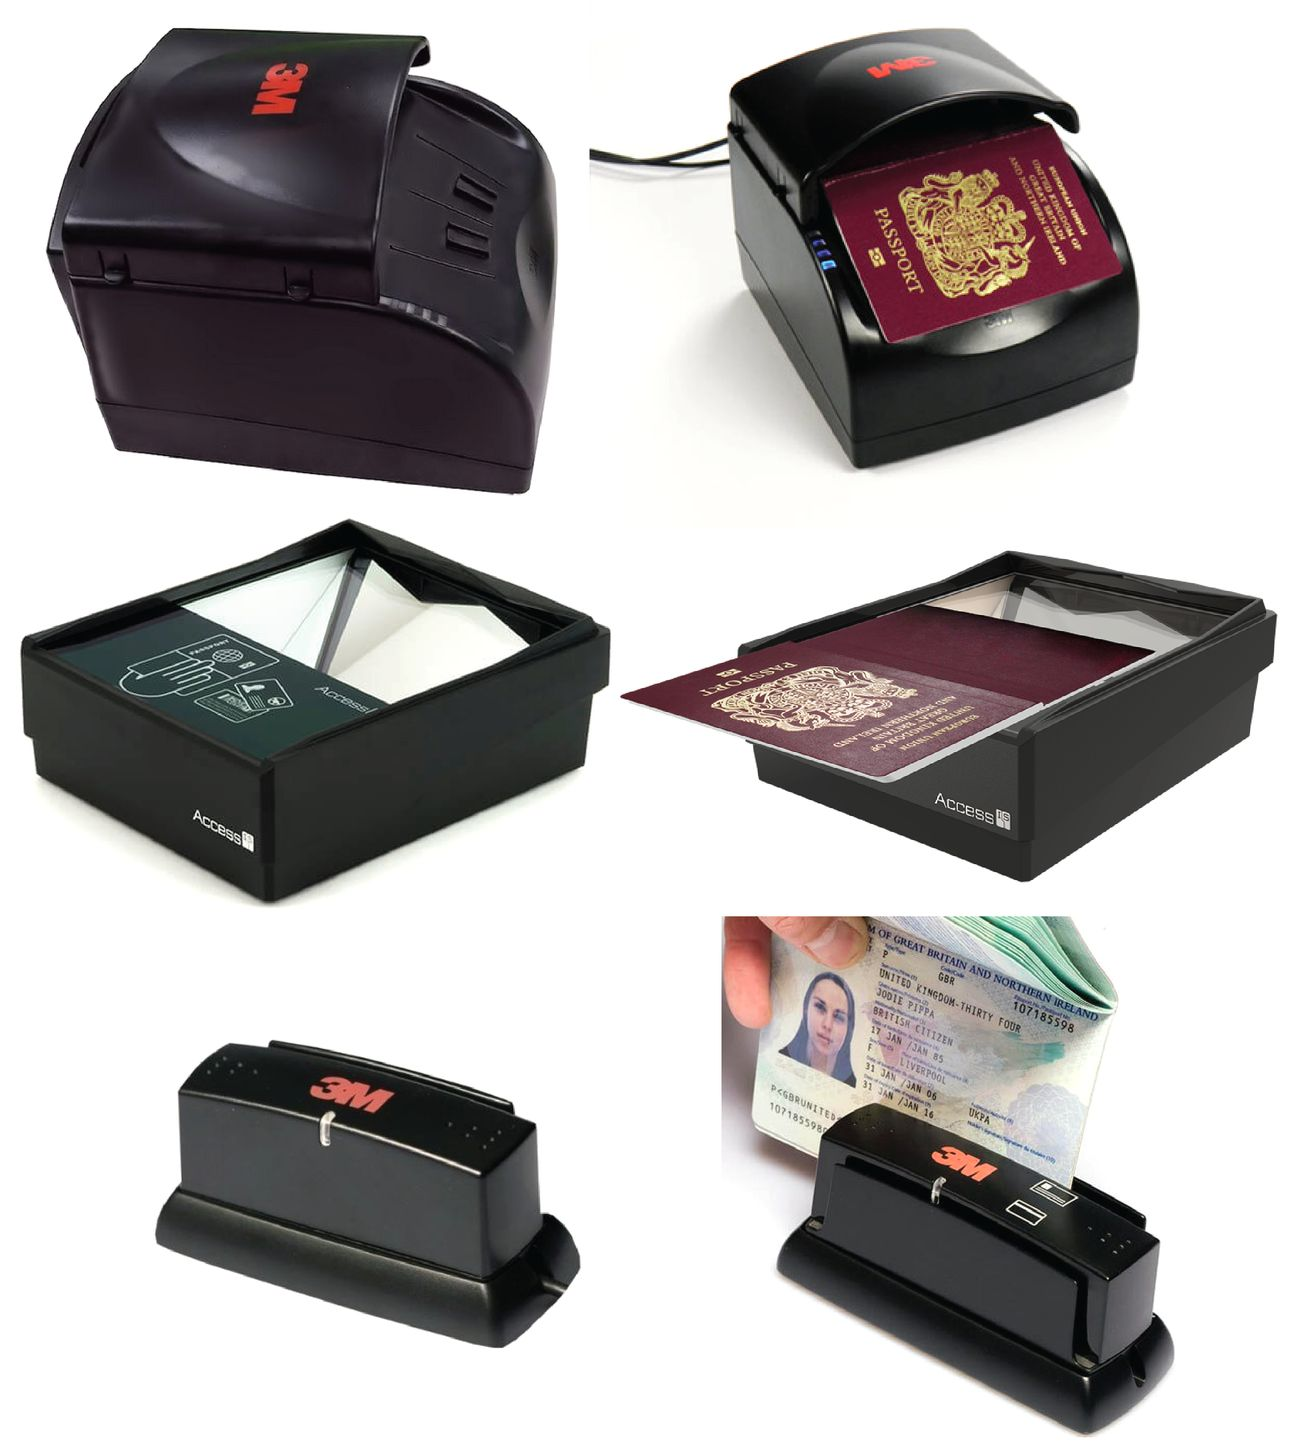
\includegraphics[width=0.5\textwidth]{ch-sistemasABC/images/ch-SistemasABC/LECTORES.png}
  \caption{Distintos tipos de lectores de \gls{eMRTD}.}
  \label{fig:lectoresDocumentos}
\end{figure}

Existen distintos tipos de lectores \GLS{eMRTD} (ver figura \ref{fig:lectoresDocumentos}), pero poder ser utilizados en sistemas \GLS{ABC} deben cumplir una serie de requisitos. \textbf{\GLS{ISO}/\GLS{IEC} $14443$} presenta un estándar para los lectores de documentos electrónicos, que al menos  debe cumplir los siguientes requisitos para poder ser homologado:

\begin{itemize}
    \item
    Debe ser capaz de leer los documentos \gls{eMRTD} definidos por \GLS{ICAO}-Doc $9303$ \cite{doc20069303}.

    \item
    Debe ser autoservicio, de fácil manejo y adaptado a personas diestras y zurdas.

    \item
    Debe tener un entrada amplia que no requiera de doblar las hojas y permita presentar el documento por la hoja de datos, donde se encuentra la zona \GLS{MRZ}, sin riesgo de deterioro.

    \item
    Debe ser capaz de escanear al menos a $385$ \gls{DPI}.
    
    \item
    Debe verificar todos los elementos ópticos de seguridad (Figura \ref{fig:MarcasSeguridadDocumentos}), por lo que es necesario que además de escanear una imagen de luz visible (\GLS{RGB}), escanee también una imagen infrarroja (\GLS{IR}) y otra ultravioleta (\GLS{UV}-A).
    
    \item
    Es recomendable que esté protegido de la luz exterior.

    \item
    Debe disponer de un módulo de lectura de radio frecuencia para poder leer el chip del \gls{eMRTD} con una velocidad mínima de $480$ Mbit/s. 

    \item
    Para conectarse con la unidad de procesos, se recomienda como mínimo una conexión USB $2.0$ a $480$ Mbits.
    
    \item
    Es recomendable que tenga una fuente de alimentación independiente al resto de sistema.

    \item
    La lectura de los datos debe realizarse en aproximadamente $2$ seg. y la verificación de los datos $8$ seg. dependiendo del número de comprobaciones con sistemas externos tengan que realizarse.

\end{itemize}


